\documentclass[11pt]{article}
\def\showsolutions{1}

\usepackage{fullpage}
%\usepackage{enumitem}
\usepackage{paralist}

\usepackage{amsmath,amsthm,amsfonts,amssymb,mathtools,latexsym}
\usepackage[dvipsnames]{xcolor}
\usepackage{graphicx,hyperref,float}
\usepackage[ruled,vlined,linesnumbered]{algorithm2e}

\usepackage{tikz}
\usetikzlibrary{trees,shapes.geometric,positioning,arrows.meta}

\usepackage{listings}

  \definecolor{customgreen}{rgb}{0,0.6,0}
  \definecolor{customgray}{rgb}{0.5,0.5,0.5}
  \definecolor{custommauve}{rgb}{0.6,0,0.8}
  
  \lstset{ 
    basicstyle=\ttfamily\footnotesize,        % the size of the fonts that are used for the code
    breaklines=true,                 % sets automatic line breaking
    commentstyle=\color{customgreen},    % comment style
    firstnumber=1,                % start line enumeration with line 1000
    frame=single,	                   % adds a frame around the code
    keepspaces=true,                 % keeps spaces in text, useful for keeping indentation of code (possibly needs columns=flexible)
    keywordstyle=\color{blue},       % keyword style
    numbers=left,                    % where to put the line-numbers; possible values are (none, left, right)
    numbersep=10pt,                   % how far the line-numbers are from the code
    numberstyle=\tiny\color{customgray}, % the style that is used for the line-numbers
    rulecolor=\color{black},         % if not set, the frame-color may be changed on line-breaks within not-black text (e.g. comments (green here))
    showspaces=false,                % show spaces everywhere adding particular underscores; it overrides 'showstringspaces'
    showstringspaces=false,          % underline spaces within strings only
    showtabs=false,                  % show tabs within strings adding particular underscores
    stepnumber=1,                    % the step between two line-numbers. If it's 1, each line will be numbered
    stringstyle=\color{custommauve},     % string literal style
    tabsize=2,	                    % sets default tabsize to 2 spaces
    title=\lstname                   % show the filename of files included with \lstinputlisting; also try caption instead of title
  }


\usepackage{array}
\usepackage{multicol}
\usepackage{booktabs}

\usepackage{hyperref}
\usepackage{cleveref}

\usepackage[ruled,vlined,linesnumbered]{algorithm2e}






\definecolor{oxblue}{RGB}{0, 30, 150}



% box around soln
\newcommand{\answerbox}[1]{\fbox{\textcolor{white}{\rule{#1}{24pt}}}}
\newcommand{\answerboxshort}[1]{\fbox{\textcolor{white}{\rule{#1}{14pt}}}}
\newcommand{\answerboxtall}[2]{\fbox{\textcolor{white}{\rule{#1}{#2}}}}


\newcommand\mycommfont[1]{\footnotesize\ttfamily\textcolor{blue}{#1}}
\SetCommentSty{mycommfont}



\pdfpagewidth 8.5in
\pdfpageheight 11in 

\oddsidemargin 0in
\evensidemargin 0in


\newtheorem{claim}{Claim}
\newtheorem{definition}{Definition}
\newtheorem{theorem}{Theorem}
\newtheorem{lemma}{Lemma}
\newtheorem{observation}{Observation}
\newtheorem{question}{Question}
\newtheorem{problem}{Problem}

\newcommand{\re}{{\mathbb{R}}}
\newcommand{\floor}[1]{\lfloor {#1} \rfloor}
\newcommand{\ceil}[1]{\lceil {#1} \rceil}
\newcommand{\paren}[1]{\left( {#1} \right)}
\newcommand{\bparen}[1]{\big( {#1} \big)}
\newcommand{\Bparen}[1]{\Big( {#1} \Big)}

\newcommand{\set}[1]{\left\{ {#1} \right\}}

\DeclareMathOperator{\E}{\mathbb{E}}
\DeclareMathOperator{\StdDev}{\mathbb{\text{\rm StdDev}}}


\newcommand{\adamnote}[1]{\marginpar{{\tiny \sf \color{orange} Adam: {#1}}}}


\newenvironment{solution}
  {\medskip\noindent\color{oxblue}}
  {\medskip}

\ifnum\showsolutions=0
    \newsavebox{\discardbox}
    \renewenvironment{solution}{\setbox\discardbox=\vbox\bgroup}
    {\egroup}
\fi 


\setlength{\parindent}{0pt}
\setlength{\parskip}{6pt}
\begin{document}
\begin{center}\Large\textbf{Homework 1}\end{center}
\section*{1. Runtime Analysis}
(a) $w = 5 \times 10^{-9}$\par
\begin{figure}[H]
\centering
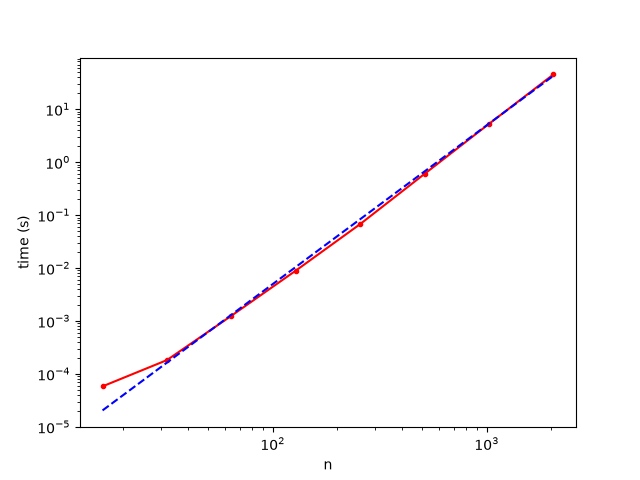
\includegraphics[width=0.9\linewidth,height=0.35\textheight,keepaspectratio]{./hw1_1_a_fig.png}
\end{figure}
(b)\par
\begin{lstlisting}[language={},columns=fullflexible]
assert a,b,c,n > 0 
assert a,b,c <= n // set bounds that a,b,c are at most n

// get the maximum numbers of each bill for the permutation
max 3 buck <- min(c,n/3)
max 2 buck <- min(b,n/2)
max 1 buck <- min(a,n)

// initialize the counter
count <- 0


for (the number of max 3 buck):
    for (the number of max 2 buck):
        if (1. (3* the number of 3 buck for each iteration) > n
            2. (2* the number of 2 buck for each iteration) > n
            3. (n - (
                    (3* the number of 3 buck for each iteration)
                    +
                    (2* the number of 2 buck for each iteration)
                    ) > n
                ) \tcc{the indentation for 3rd condition is merely for the better readability.}
            ):
            do nothing and move on
        else:
            add 1 to count

return count         
\end{lstlisting}
Proof:\par
Let \texttt{a} and \texttt{b} be the number of 3-buck and 2-buck coins to be combined.\par
Let \texttt{A} be a 2D array that contains all sums of permutations of \texttt{a} AND \texttt{b} that those sums are always less than or equal to \texttt{n}.\par
So, the number of possible permutations is $a \times b$ and the runtime is $O(n^2)$.\par
If we add another condition that filters whether the value of each sum in \texttt{A} subtracted by \texttt{n} does not exceed the maximum number of 1-buck coin provided, we can calculate all the possible permutation and how many the permutations there are at the same time in $n^2$ times.\par

Hence, the asymptotic coin choice algorithm can have time complexity of $O(n^2)$.\par

Runtime Analysis:\par
1. Variable initialization: the maximum number of coins we can combine and counter $O(1)$\par
\begin{lstlisting}[language=Java,columns=fullflexible]
int max_three_buck = Math.min(c, n/3);
int max_two_buck = Math.min(b,n/2);
int max_one_buck = Math.min(a,n);
int count = 0;
\end{lstlisting}

2. Main Loop: $O(n^2)$\par
1) iterate through the maximum numbers of three-buck and two-buck coin ($O(n^2)$)\par
2) eliminate the possible permutations that would go out of bounds from the counter\par
2-1. if the given number of 3-buck coins worth more than n\par
2-2. if the given number of 2-buck coins worth more than n\par
2-3. if the given number of 3-AND-2-buck coins(permutation) worth more than n\par
2-4. From the permutation without 2-1,2,3., if the left-over money is greater than the maximum number of 1-buck coin.\par
2-5. Otherwise, put it in the counter.\par
3) Return the number of permutations ($O(1)$)\par
\begin{lstlisting}[language=Java,columns=fullflexible]
for (int first = max_three_buck; first >= 0; first--){
    for (int second = max_two_buck; second >= 0; second--){
        if(3*first > n||2 * second > n || (3*first)+(2*second) > n || (n-(2*second+3*first)) > max_one_buck){
            continue;
        } else {
            count++;
        }
    }
}
\end{lstlisting}
3. Return result: $O(1)$\par
\begin{lstlisting}[language=Java,columns=fullflexible]
return count;
\end{lstlisting}

Complete Runtime = $O(1)$ + $O(n^2)$ + $O(1)$ = $O(n^2)$\par
Therefore, the runtime of this asymptotically faster algorithm for this problem is $O(n^2)$.\par
(c)\par
\begin{figure}[H]
\centering
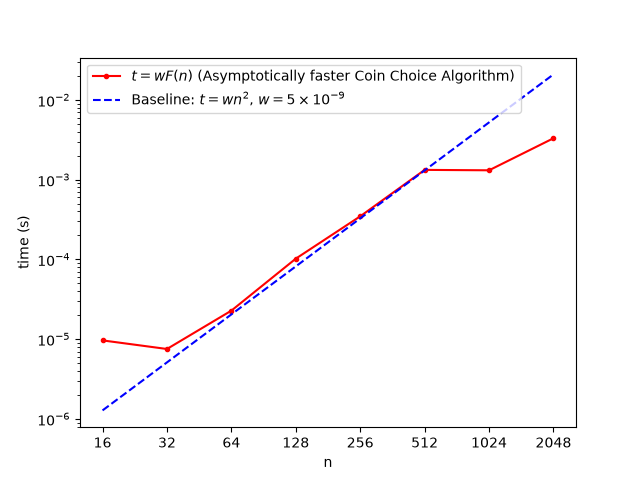
\includegraphics[width=0.9\linewidth,height=0.35\textheight,keepaspectratio]{./hw1_1_c_fig.png}
\end{figure}
Initially, \texttt{w} value was $5 \times 10^{-8}$ as default. For part (a), I changed the exponent to $-9$, which fits to the original algorithm with time complexity of $O(n^3)$. For the part (c), I did not change \texttt{w} value and still able to fit my asymptotically faster algorithm with time complexity of $O(n^2)$. Because \texttt{w} value is just an adjustment parameter to make the comparison between the baseline $t=wn^2$ and my algorithm human-friendly and my hardware setup was not changed, I did not have to change \texttt{w} value from part (a). One problem I encountered was the data extraction. Since I wrote the algorithm in Java and the original algorithm is in python, I had to come up with an idea that I can put into the plot in python (I don't know how to plot in Java so I had to extract data that can be read cross-linguistically.)\par
\end{document}
